\chapter{Reasoning about fault activation}
\label{chap:activation}

The \ac{activation} proposed in this work emerges from the need to analyse the behaviour of a system when a subset of the faults have been triggered in some order, and to provide completeness analysis of system behaviour.
%
There are at least two strategies to use \ac{activation} to obtain structure expressions of \ac{SFT}, \ac{TFT}, or \ac{DFT}: 
\begin{alineasinline}
  \item model systems directly in \ac{activation}, and 
  \item obtaining operational mode expressions extracted from failure traces, as shown in the work reported in~\cite{DM2016}.
\end{alineasinline}
%
In approaches as those reported in~\cite{WP2009,Merle2010}, behavioural completeness is left for the analyst.
Using tautology and the indication of undefined nominal values, we ensure that no situation is missed.
That is, modelling is behaviourally complete.

The \acl{activation} associates: 
\begin{alineasinline}
  \item an operational mode, and 
  \item the expression of fault events that \emph{activates} the operational mode or error event.
\end{alineasinline}
The expressions of fault events can be written in any algebra that provides tautology and contradiction properties.
Boolean algebra and \ac{algebra} provide both.
Thus, \ac{activation} is parametrized by: 
\begin{alineasinline}
  \item an algebra that provides at least tautology and contradiction, and 
  \item operational modes.
\end{alineasinline}
\Cref{fig:logic-overview} depicts an overview of \ac{activation}.
%
\begin{figure}[ht]
  \centering
  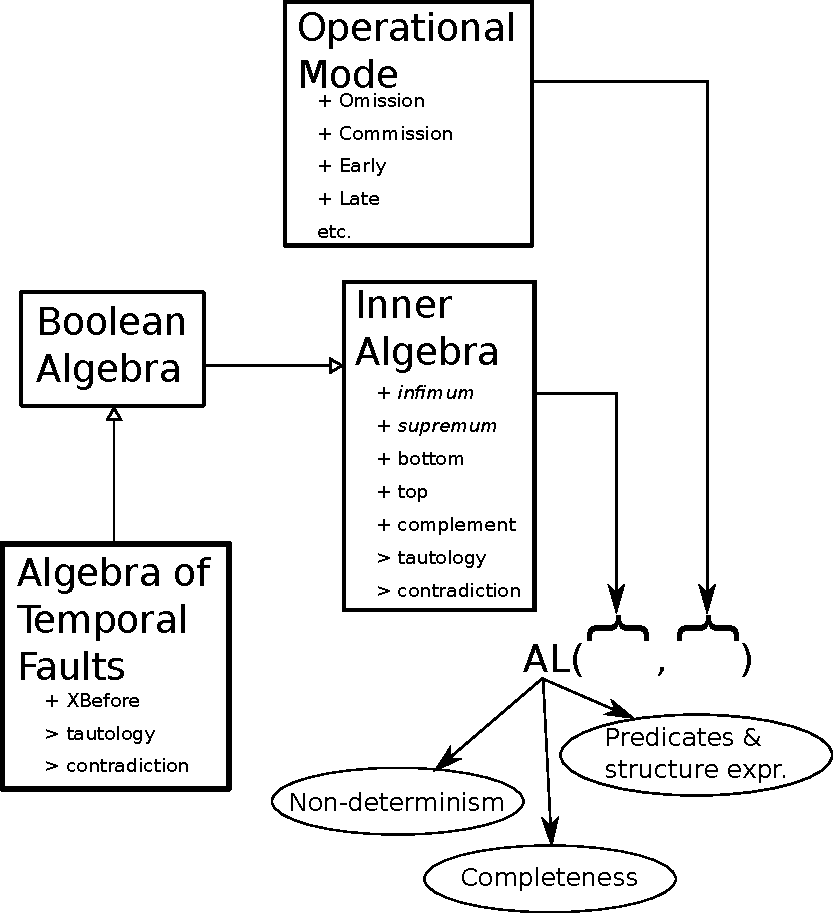
\includegraphics[width=0.6\textwidth]{logic-overview}
  \caption{\Ac{activation} overview}
  \label{fig:logic-overview}
\end{figure}

%Finally, structure expressions with order-related operators can be complex to analyse.
%Even to determine whether they are a contradiction or not~\cite{WP2009}.

%For example, what is the system behaviour when fault A occurs and then fault B occurs?
%What is a component behaviour when it detects a faulty behaviour in some of its inputs?
%Or, does the analyst considered all possibilities?
%Is there any erroneous behaviour case missing?

\begin{sloppypar}
We summarise the properties of \ac{activation} as follows:
%
\begin{enumerate}
  \item No expression predicate is a contradiction: there are no \emph{false} predicates in activation expressions;
  %\item There are no two terms that are \emph{active} simultaneously: only explicit non-determinism is allowed;
  \item The predicates in the terms of an expression consider all possible situations: expression tautology;
  \item There are no two terms with exactly the same operational mode: all expression terms are related to a unique operational mode.
\end{enumerate}
%
These properties form the \emph{healthiness conditions}~\cite{HH1998} of an expression in \ac{activation}.
\end{sloppypar}

We show the general form of \ac{activation} to model faults in \cref{sec:grammar}, the healthiness conditions to normalize expressions in \cref{sec:healthiness-conditions}, how to identify non-determinism in an expression in \cref{sec:non-determinism}, and the predicate notation to analyse systems and model fault propagation in \cref{sec:predicates-notation}.

\section[The Activation Logic Grammar]{The \acl*{activation} Grammar}
\label{sec:grammar}

Each term in \ac{activation} is a pair of a predicate and an operational mode.
The predicate is written in either Boolean algebra, \ac{algebra}, or any algebra that provides these properties: tautology and contradiction.
We assume that the set of possible faults on a system is finite and that each variable declared in a predicate represents a fault event.

The operational mode has two generic values: 
\begin{alineasinline}
  \item Nominal, and 
  \item Failure.
\end{alineasinline}
Nominal values either determine a value, or an undefined value (in this case, the constant value ``$\undefinednominal$'' is assumed).
Failure values denote an erroneous behaviour, which can be a total failure (for example, signal omission) or a failure that causes degradation (for example, a signal below or above its nominal range).
The choice of the operational modes depends on the system being analysed and its definition is generic and is left for the analyst.
For the \ac{activation}, it is sufficient to specify that it is an erroneous behaviour.

The grammar is parametrized by the syntax of an algebra (\verb|Algebra|) and a set of operational modes (\verb|OperModes|).
The initial rules of the grammar are defined as follows:
\begin{verbatim}
AL(Algebra, OperModes)     = TERM(Algebra, OperModes) 
                             | TERM(Algebra, OperModes) 
                               `|' AL(Algebra, OperModes)
TERM(Algebra, OperModes)   = `(' Algebra `,' OM(OperModes) `)'
OM(OperModes)              = `Nominal' NominalValue 
                             | `Failure' OperModes
NominalValue               = `undefined' | Number
Number                     = Integer | Bool | Decimal
\end{verbatim}
%
The denotational semantics of the expressions in \ac{activation} is a set of pairs.
The predicate in each term of an expression depends on the semantics of the inner algebra.
Thus the predicate evaluates to either \emph{true}~($\top$) or \emph{false}~($\bot$) depending on the valuation in the algebra.
In what follows we show a sketch of the denotational semantics of \ac{activation}.
%
\begin{align*}
  \logicInFormula{\left(P_1, O_1\right)} &\mapsto \{\left(P_1, O_1\right)\}\\
%%%%%%%%%%%%%%%%%%%%%%%%%%%%%%%%%%%%%%%%%%%%%%%%%%%%%%%%%%%%
  \logicInFormula{\left(P_1, O_1\right) | \left(P_2, O_2\right)} &\mapsto
    \{\left(P_1, O_1\right), \left(P_2, O_2\right)\}\\
%%%%%%%%%%%%%%%%%%%%%%%%%%%%%%%%%%%%%%%%%%%%%%%%%%%%%%%%%%%%
  \logicInFormula{Nominal~100} &\mapsto \Nominal{100}\\
%%%%%%%%%%%%%%%%%%%%%%%%%%%%%%%%%%%%%%%%%%%%%%%%%%%%%%%%%%%%
  \logicInFormula{Nominal~undefined} &\mapsto \Nominal{\undefinednominal}\\
%%%%%%%%%%%%%%%%%%%%%%%%%%%%%%%%%%%%%%%%%%%%%%%%%%%%%%%%%%%%
  \logicInFormula{Failure~Omission} &\mapsto \Failure{Omission}
\end{align*}
%
In an expression, if the $i^{th}$ predicate evaluates to $true$ ($\top$), we say that the $i^{th}$ operational mode is \emph{activated}.
To simplify the presentation of the expressions and to ease understanding, we use the denotational semantics in the remainder of this chapter (the right-hand side of the sketch above).
Thus, instead of using $\logicInFormula{Exp} = \logicInFormula{\left(P_1,O_1\right)} | \logicInFormula{\left(P_2,O_2\right)}$ we use $Exp = \left\{ \left(P_1,O_1\right), \left(P_2,O_2\right)  \right\}$

In this \lcnamecref{sec:grammar}, to illustrate the properties and possible analyses, we use an example of a system with faults $A$ and $B$ and the following outputs:
\begin{description}
  \item[$O_1$:] when $A$ is active;
  \item[$O_2$:] when $B$ is active;
  \item[$O_3$:] when $A$ is active, but $B$ is not;
  \item[$O_4$:] when $A$ or $B$ are active.
\end{description}
%
The expression for this example in \ac{activation} is:
\begin{equation}
S = \left\{\left(A, O_1\right), \left(B, O_2\right), \left(A \land \lnot B, O_3\right), \left(A \lor B, O_4\right)\right\}\label{eq:activation-example}
\end{equation}
%
We use \cref{eq:activation-example} in the following sections of this chapter to illustrate \ac{activation}.

In this example we see that one of the healthiness conditions is not satisfied: when, for instance, $A$ and $B$ are both inactive ($\lnot \left(A \land B\right)$), there is no explicit output defined.
%
In \cref{sec:activation-to-structure-expressions-algebra-operators} we show a more detailed case study to illustrate the reasoning about temporal faults.
In the next \lcnamecref{sec:healthiness-conditions}, we show how to normalise the expression, so that the three healthiness conditions are satisfied.

\section{Healthiness Conditions}
\label{sec:healthiness-conditions}

The healthiness conditions are fix points of a language.
The property is defined as a function of an expression and returns another expression.
For example, if a healthiness condition $\healthiness$ is satisfied by an expression $Exp$, we have $\healthinessfun{Exp} = Exp$.

In what follows we show the three healthiness conditions for \ac{activation}.
For convenience, we use the following abbreviations:
\begin{description}
  \item[contradiction:] the expression always evaluates to \emph{false};
  \item[tautology:] the expression always evaluates to \emph{true}.
\end{description}

\subsection[H1: No predicate is a contradiction]{$\healthiness[1]$: No predicate is a contradiction}
\label{sec:h1}

This property is very simple and it is used to eliminate any term that has a predicate that always evaluates to false.

\begin{definition}
Let $exp$ be an expression in \ac{activation}, then:
%
\begin{equation}
\healthinessfun[1]{exp} = \left\{~\left(P,O\right) ~|~ \left(P,O\right) \in exp \land \lnot \contradiction{P} ~\right\}
\end{equation}
%
where the operator $\in$ indicates that a term is present in the expression.
\end{definition}

Applying the first healthiness condition to our example results in:
\[\healthinessfun[1]{S} = S\]

Thus, we conclude that $S$ \emph{is} $\healthy[1]$.

\subsection[H2: All possibilities are covered]{$\healthiness[2]$: All possibilities are covered}
\label{sec:h2}

This property is used to make explicit that there are uncovered operational modes.
In this case, there is a combination of variables in the algebra that was not declared in the expression.
Very often the focus when modelling faults is on erroneous behaviour.
So we assume that such an uncovered operational mode is nominal, but has an undefined value.

\begin{definition}
Let $exp$ be an expression in the \ac{activation}, and $\tau$ is:
\[
\tau = \lnot \left (\bigvee_{\left(P,O\right)\in exp} P\right)
\]
%
then:
%
\begin{equation}
\healthinessfun[2]{exp} = 
  \begin{cases}
    exp, & \text{if } \contradiction{\tau}\\
    exp \cup \left\{\left(\tau,\Nominal{\undefinednominal}\right)\right\}, & \text{otherwise}
  \end{cases}
\end{equation}

\end{definition}

This property checks erroneous behaviour completeness. 
If the expression is already complete, all possibilities are already covered, and the expression is healthy.
Otherwise, a term containing the missing terms is introduced using the $\Nominal{\undefinednominal}.$

Applying the second healthiness condition to our example results in the following expression after simplification:
\[\healthinessfun[2]{S} = S \cup \left\{\left(\lnot A \land \lnot B, \Nominal{\undefinednominal}\right)\right\}\]

Thus, we conclude that $S$ \emph{is not} $\healthy[2]$.

\subsection[H3: There are no two terms with exactly the same operational mode.]{$\healthiness[3]$: There are no two terms with exactly the same operational mode}
\label{sec:h3}
This property merges terms that contain the same operational mode.
It avoids unnecessary formulas and may reduce the expression.

\begin{definition}
Let $exp$ be an expression in \ac{activation}. Then:
%
\begin{equation}
\label{eq:h3}
\begin{split}
\healthinessfun[3]{exp} = \left\{ \right.&\left(P_1, O_1\right) | \left(P_1, O_1\right) \in exp ~\land \\
    &\forall \left(P_2,O_2\right) \in exp \bullet 
      \left(P_1, O_1\right) = \left(P_2, O_2\right) \lor O_1 \neq O_2
  \left.\right\} \cup \\
  & \left\{ \left(P_1 \lor P_2, O_1\right) | \left(P_1, O_1\right),\left(P_2, O_2\right) \in exp \land O_1 = O_2 \right\}
\end{split}
\end{equation}
\end{definition}

Applying $\healthiness[3]$ in the example in the beginning of the \lcnamecref{chap:activation}, we conclude that $S$ \emph{is} $\healthy[3]$.
On the other hand, if we consider an $S'$ system being a copy of $S$, but making $O_1 = O_2$, then:
\[
\healthinessfun[3]{S'} = \left\{ 
  \left(A \lor B, O_1\right),
  \left(A \land \lnot B, O_3\right),
  \left(A \lor B, O_4\right)
\right\}
\]
Thus, we conclude that $S'$ \emph{is not} $\healthy[3]$.

\subsection{Healthy expression}
\label{sec:h}

To obtain a healthy expression, we apply all three healthiness conditions.
The order of application of each healthiness condition does not change the resulting expression.
The healthiness function is written as the composition of functions as follows:
\begin{equation}
\label{eq:h}
\healthiness = \healthiness[1] \circ \healthiness[2] \circ \healthiness[3]\end{equation}

After applying the three healthiness conditions to $S$, the resulting expression is:
\[
\begin{split}
\healthinessfun{S} = \left\{\right.
  & \left(A, O_1\right), \left(B, O_2\right),\\
  & \left(A \land \lnot B, O_3\right), \left(A \lor B, O_4\right),\\
  & \left(\lnot A \land \lnot B, \Nominal{undefined}\right)
\left.\right\}
\end{split}
\]

The healthiness conditions are useful to faults modelling, aiding the faults analyst to check contradictions and completeness.
Also, obtaining safe predicates is only possible in healthy expressions.
In the next \lcnamecref{sec:non-determinism}, we show how to verify non-determinism in \ac{activation} expressions.


\section{Non-determinism}
\label{sec:non-determinism}

Non-determinism is usually an undesirable property.
Thus, the analysis shall consider the activation of faults even if the fault might or not be active.

To identify non-determinism, we can check for the negation of a contradiction in a pair of predicates in the algebra.

\begin{definition}[Non-determinism]
\label{def:non-determinism}
Let $exp$ be an expression in \ac{activation}.

\begin{equation}
\label{eq:non-determinism}
\begin{split}
\nondet{exp} = &~ \exists \left(P_1,O_1\right),\left(P_2, O_2\right) \in exp~\bullet \\
  &~ \lnot \contradiction{P_1 \land P_2}
\end{split}
\end{equation}

\end{definition}

If there is at least one combination that evaluates $P_1 \land P_2$ to true (it is not a contradiction), then $exp$ is non-deterministic.
Our example is clearly non-deterministic as at least $A \land \left(A \lor B\right)$ is not a contradiction.

To analyse components and systems, and to model faults propagation, a predicate notation is shown in the next \lcnamecref{sec:predicates-notation}.
The predicate notation offers two additional ways to check non-determinism.

\section{Predicate Notation}
\label{sec:predicates-notation}

The \acl{activation} needs a special notation to enable the analysis of: 
\begin{alineasinline}
  \item a particular faults expression, or 
  \item a propagation in components.
\end{alineasinline}
Such a special notation extracts predicates in the algebra given an observable failure of the system (an undesired operational mode).

\begin{definition}[Predicate]
\label{def:predicate}
Let $exp$ be an expression in \ac{activation}, and $O_x$ an operational mode.
A predicate over $exp$ that matches $O_x$ is described as:
\begin{equation}
\label{eq:predicate}
\predicate{exp}{O_x} \iff \left.\exists \left(P, O\right) \in \healthinessfun{exp}\ \middle|\ O = O_x \bullet P\right.
\end{equation}
\end{definition}


The predicate notation function returns a predicate in the algebra.
For the example in the beginning of this \lcnamecref{sec:predicates-notation}, the predicate for $O_2$ is obtained as follows:
\[
\predicate{S}{O_2} = B
\]

To allow fault propagation of components we need another special notation. 
It expands the modes of an expression with a predicate in the inner algebra.

\begin{definition}[Modes]
Let $exp$ be an expression in \ac{activation}, and $P$ a predicate in the inner algebra, then:
\begin{equation}
\label{eq:modes}
\modes{exp}{P} = \left\{ \left(P_i \land P, O_i\right)\ \middle|\ (P_i, O_i) \in \healthinessfun{exp} \right\}
\end{equation}
%\begin{align*}
%\modes{S}{P} = &~ 
%	\left\{
%		\left(A \land P, O_1 \right), 
%		\left(B \land P, O_2 \right), 
%		\left(A \land \lnot B \land P, O_3 \right), 
%		\left(\left(A \lor B\right) \land P, O_2 \right)
%	\right\}
%\end{align*}

\end{definition}

Finally, to check the possible outputs, we need a function to obtain a set of outputs given an expression.

\begin{definition}[Activation]
\label{def:activation}
Let $exp$ be an expression in \ac{activation}, and $P_x$ a predicate in the inner algebra, then:

\begin{equation}
\label{eq:activation}
\activation{exp}{P_x} = \left\{
    O | (P, O) \in \healthinessfun{exp} \land \tautology{P_x \implies P}
  \right\}
\end{equation}

\end{definition}

Non-determinism can also be checked using the predicate notation and the activation property:
\begin{subequations}
\begin{align}
\activation{S}{A \land \lnot B} = &
  \left\{O_1, O_3\right\}\label{eq:s-nondet-activation}\\
\predicate{S}{O_1} \land 
  \predicate{S}{O_3} = & A \land \lnot B\label{eq:s-nondet-pred}
\end{align}
\end{subequations}
%
\Cref{eq:s-nondet-activation} shows that both $O_1$ and $O_3$ can be observed if $A \land \lnot B$ is \emph{true}. 
\Cref{eq:s-nondet-pred} states that if the possible operational modes of healthy $S$ are $O_1$ and $O_3$, then the predicate is $A \land \lnot B$.
Non-determinism is the possibility of observing two different failures ($O_1$ and $O_3$) for the same failure expression ($A \land \lnot B$) in the algebra.
In the next \lcnamecref{chap:case-study}, we show a practical case study using these properties and notations.

